\section{Protocol Implementations}
\subsection{Diffie-Hellman-Merkel}
In this section we will implement a Echo server that uses the Diffie-Hellman-Merkle key exchange to secure the communication channel. The focus of the implementation will not be on the actual encryption of values and strength of keys. We will however focus on how you would create a basic system that can later be expanded. The reason for this is that DHM requires numbers in the size of over 1024 bits to truely be secure. Implementing our solution for this would shift the focus too much on the cryptography aspect rather than the implementation. In  a real world application one would want to use a cryptographic library to handle the generation of these security elements. We have opted to create our own simple methods instead of adding these libraries.

\subsubsection{Specifying the protocol}
The basis of our design will be entirely dependant on the protocol definition. It seems only natural to start the design process here.

\subsubsubsection{JSON}
For this implementation we will use the JSON format for sending and receiving messages. Although our solution can work with any type of message, we find JSON to be easily readable and understandable.
\subsubsubsection{Protocol}
We have written about the Diffe-Hellman-Merkle key exchange in \ref{sec:dhm} Diffie-Hellman-Merkel on page \pageref{sec:dhm}. The key elements of this protocol is Alice starting a communication with Bob by sending a prime Number and generator, message 1. Many real-world implementations use pre-defined generators, but we will allow the generator to be dynamic for our implementation. After Bob receives this message, he sends to Alice his public key. The final step then is for Alice to send her public key. After this the communication can now be encrypted using the key generated by both Alice and Bob.
\\ 
Below we have specified this part of the protocol in our DSL.
\begin{lstlisting}[style=myScalastyle]
 val endpoint = new ProtocolBuilder()
 val aliceDHM = endpoint sends primeAndGenerator 
                  receives aPublicKey sends aPublicKey
 val bobDHM   = endpoint receives primeAndGenerator 
                  sends aPublicKey receives aPublicKey
\end{lstlisting}
The only part missing now is that we want Bob to echo messages sent by Alice. We want Alice to send as many messages as she wants. We have two options to solve this. As the message sent from Alice is encrypted, the validator will not be able to verify the message. Depending on the level of security desired, we can either encrypt the entire message or only the values. To increase clarity in the system, it id beneficial to use the DelayedValidation class. This will help decrease the complexity of the implementation.

\begin{lstlisting}[style=myScalastyle]
 val aliceEcho = endpoint sends anEchoMessage 
                  receives anEchoMessage looped()
 val bobEcho   = endpoint receives anEchoMessage
                  receives anEchoMessage looped()
\end{lstlisting}

Now that we have the two parts of the protocol defined, we can combine them.
\begin{lstlisting}[style=myScalastyle]
 val aliceComplete = aliceDHM next( aliceEcho )
 val bobComplete   = bobDHM next( bobEcho )
\end{lstlisting}
The method ``next'' is a method that allows us to combine two separate ProtocolBuilders. It is useful for when we want to limit the scope of a loop step. In other words the protocol could of been written in a single line by using ``next'' to separate the ``looped()'' step from the DHM steps.
\\
Now we need to create the validators that will be used to verify the messages sent and received.

\subsubsection{Implementing Validators}
From looking at the Protocol specification from the previous section we can determine the classes that are needed. The classes that we create in this section will be sent to the consumer and can be considered as message classes. The consumer will based its response by using pattern matching on the message.
\\
We will not show how to create each class and validator, but show how we could handle the first message of the protocol.
\subsubsubsection{Prime and Generator}
\begin{lstlisting}[style=myScalastyle]
 case class PrimeAndGenerator(prime: Double, generator: Double)
\end{lstlisting}
A ``Case'' class gives us by default an immutable class, ``prime'' and ``generator'' are declared as ``val''s . This is very useful for when we pass messages to our Consumer as it ensures that the message is never mutated while en-route.
\\\\
The JSON representation of this class with the values of (7.0 , 2.0) would be the following:
\begin{lstlisting}[style=myScalastyle]
{
    "type": "PandG",
    "prime": "7.0",
    "generator": "2.0"
}
\end{lstlisting}
In the example below we have used a library that helps us extract JSON information out of a string. 

\begin{lstlisting}[style=myScalastyle]
  val primeAndGenerator = new Validator(input => try {
  val json = parse(input)
  val p = json \ "prime"  
  val g = json \ "generator"
  Right(PrimeAndGenerator(prime = p, generator = g))
  } catch {
    case e: Exception =>
      Left("Msg could not be converted to a 
              PrimeAndGenerator class: " + e.getMessage())
  })
\end{lstlisting}
Here we can see that given any form of exception, we will return a Left value with an error message. Otherwise we will return a Right value with a PrimeAndGenerator instance.

\subsubsection{Consumer}
As we have stated before, the Consumer will use pattern matching when receiving messages. All that is needed to do here is implement a response for each message. In the example below we will not show the details. 
\\
All actors must have a ``Receive'' method that handles received messages. 
\begin{lstlisting}[style=myScalastyle]
def receive = {
    case PrimeAndGenerator(prime, generator) =>
      // Generate our PrivatKey and send it
    case PublicKey(key) =>
      // Calculate the session key
    case EchoMessage(message) =>
      // Return message
    case ProtocolEnded(reason) =>
      // Protocol has ended due to 'reason'
      // Tell PM it is safe to quit
    case _ =>
      // Unknown message received
}
\end{lstlisting}
Shown above is the consumers ``receive'' method that deals with the various message cases. All that is missing from the implementation is calculating the $SecretKey$ and echoing encrypted messages.

\subsection{HTTP Server}
\label{sec:httpserver}
The perhaps most widely used protocol in use today is the HTTP protocol \cite{fielding1999hypertext}. It is mostly used to serve web-pages to browsers. We will in this section create a very simple web server that can serve HTML pages.

\subsubsection{Specifying the protocol}
One of the main difficulties when implementing the HTTP is that unlike our DHM protocol, there is much more information that needs to be wraped in messages. Many of these fields are optional and can be sendt in any order. These optional fields make it much more difficult for us to know what information our consumer will have avaiable when generating a response.

Below we have an example of the fields, HTTP headers are.
\begin{lstlisting}[style=myScalastyle]
  GET / HTTP/1.1
  Host: localhost:8888
  Connection: keep-alive
  Cache-Control: max-age=0
  Accept: text/html
  User-Agent: Mozilla/5.0 (X11; Linux x86_64) AppleWebKit/537.36 (KHTML, like Gecko) Chrome/43.0.2357.81 Safari/537.36
  DNT: 1
  Accept-Encoding: gzip, deflate, sdch
  Accept-Language: en-US,en;q=0.8,no;q=0.6
\end{lstlisting}
Our DSL is able to handle that these fields are optional and allowed to be in any order. The only required field is the ``GET'' line. It conveyes the purpose of the message while the other fields are supplementary information for the request.
\begin{lstlisting}[style=myScalastyle]
val httpServer = endpoint receives RequestHeaders sends 
                           ResponseHeaders 
\end{lstlisting}
Due to time constraints, our server does not run any validation on the ResponseHeaders.
\subsubsection{HTTP server running}
Here we can see the index page of our server. We also provide additional pages such as ``test1'' and ``test2''
\begin{figure}[h]
	\centering
	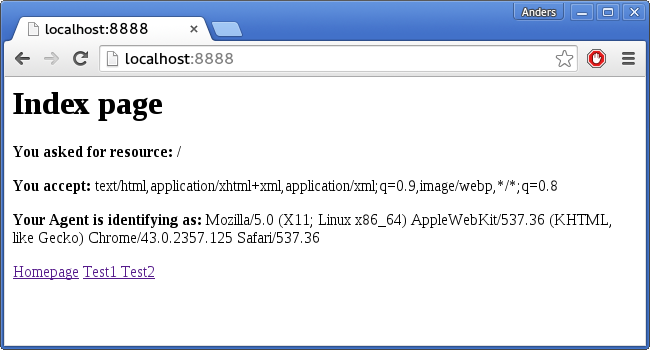
\includegraphics[scale=0.7]{images/protocolimplementations/httpserver.png} 
	\caption{HTTP Server index page}
	\label{fig:httpserver}
\end{figure}











